\chapter{検証フレームワークActario}
\label{chapter:overview}

本章では、本研究で作成したアクターシステムの検証フレームワークActarioについての概要を説明する。
Actarioでは、

\section{概要}

図~\ref{img:overview:workflow}は、Actarioを用いてアクターシステムを検証する際のワークフローである。
まずActarioが提供するアクターシステムを記述するための記法を使って、検証したいアクターシステムを記述する。
次にそのアクターシステムが満たしているべき仕様を記述し、それをActarioが提供する証明の機構によって証明する。
最後にActarioが持つErlangへのコード抽出機を用いて実装をErlangに抽出する。

\begin{figure}[tp]
  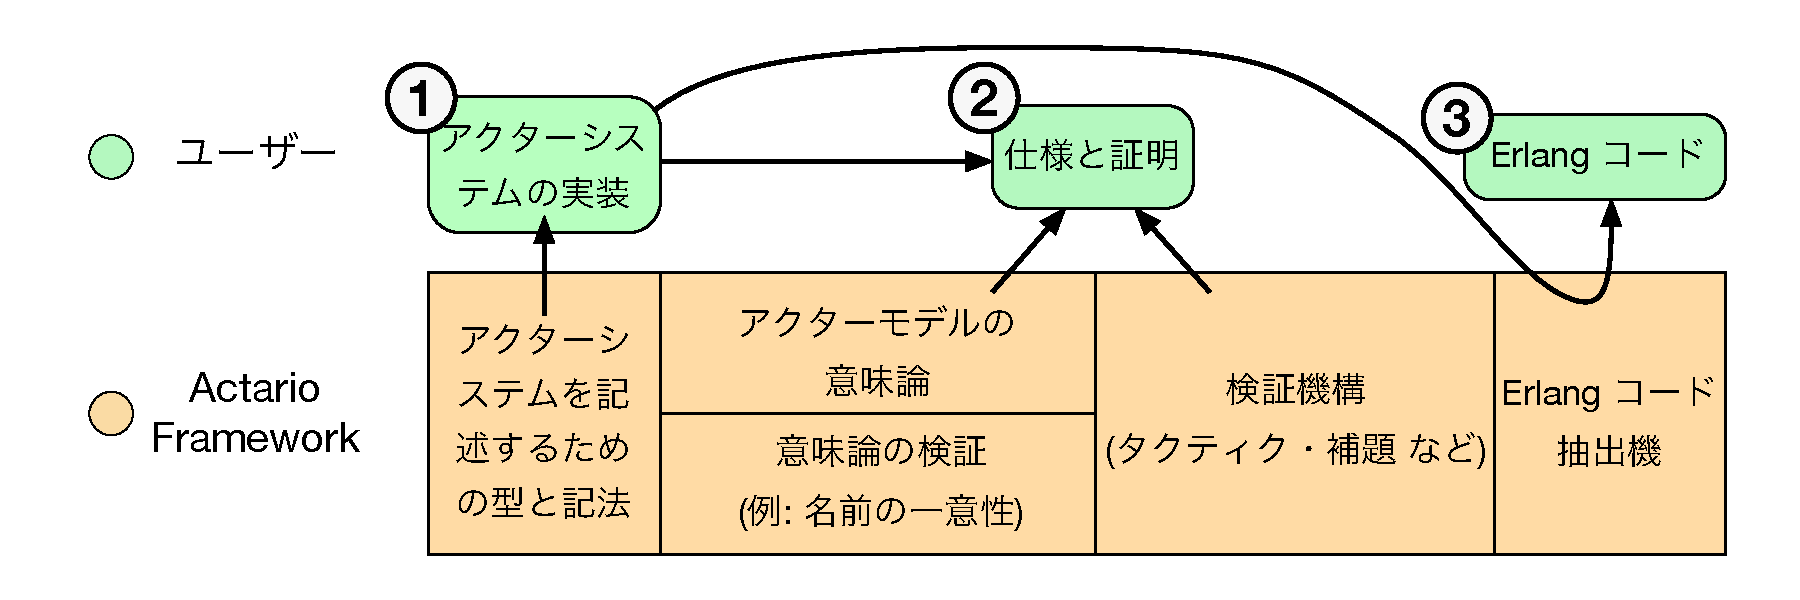
\includegraphics[width=14cm]{./img/overview/workflow.pdf}
  \label{img:overview:workflow}
  \caption{Actarioのワークフロー}
\end{figure}

\section{例:階乗計算アクターシステム}

例として、階乗を計算するアクターシステムを考える。
このシステムをActarioで記述し、仕様および証明を記述することで、
Actarioを実際にどのように使うかを説明する。

\subsection{システムの実装}

このアクターシステムは、単に一つのアクターのなかで階乗を計算するのではなく、
次に何の数を掛けるかという継続を持っているアクターを生成しながら、
階乗を計算する。(?)
図~\ref{img:overview:fact}はこのアクターシステムに$3$を与えたときの動きを表した図である。

\begin{figure}[tp]
  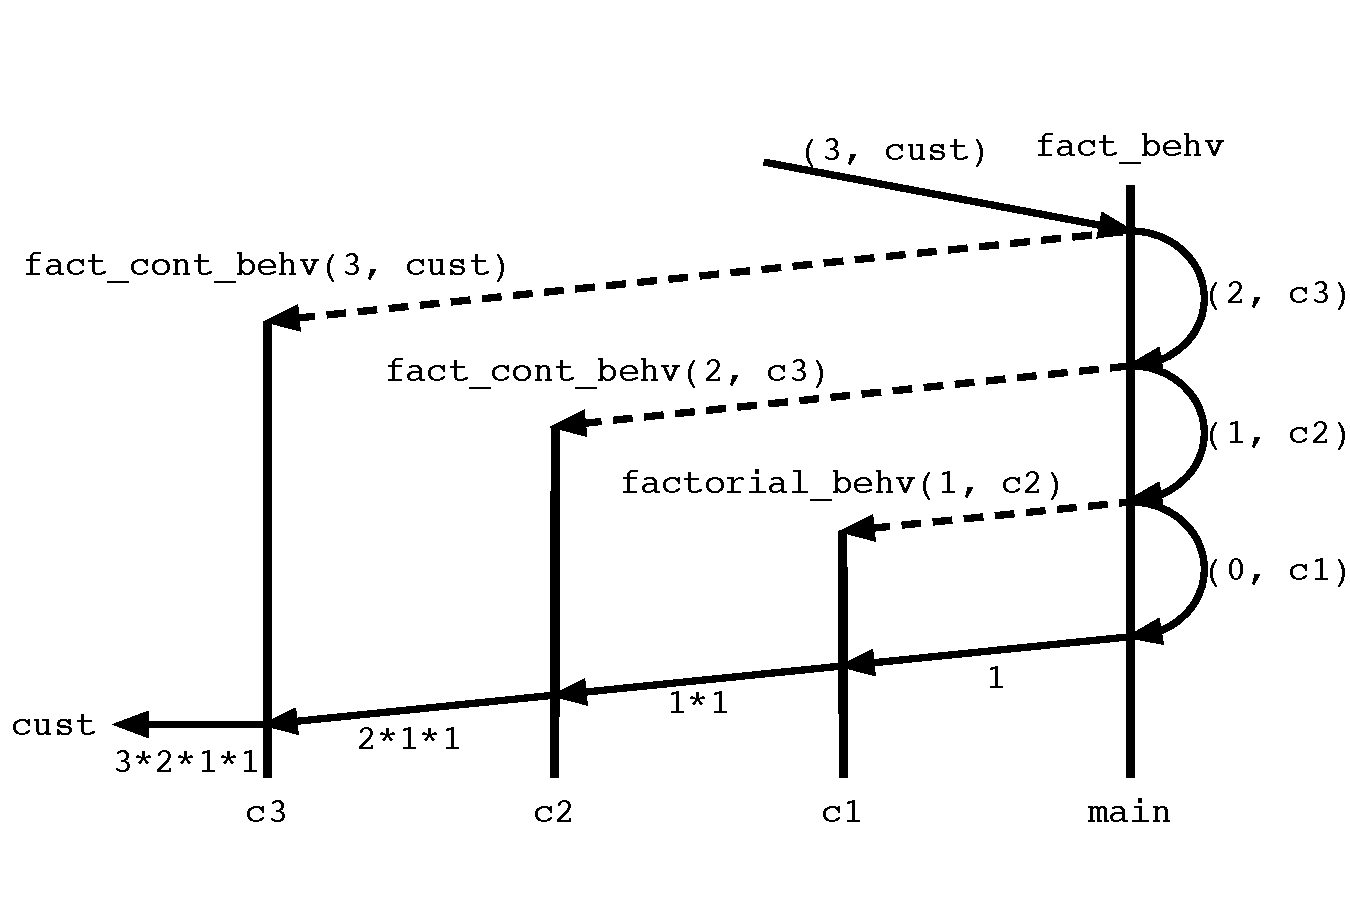
\includegraphics[width=14cm]{./img/overview/fact.pdf}
  \label{img:overview:fact}
  \caption{fact 3}
\end{figure}

Actarioを用いると階乗計算アクターシステムは図~\ref{code:overview:fact-impl}のように記述することができる。
\texttt{factorial\_cont\_behv}は継続を保持しているアクターの振る舞いのテンプレートである。
保持する数と計算結果を渡すアクターの名前を受け取り、アクターの振る舞いとなる。
このアクターは、メッセージを受け取った際にそれが数なら保持している数\texttt{val}と掛けあわせ、
計算結果を待ち受けているアクター\texttt{cust}に送信する。
送信後は何もしないアクターとなる。
次の\texttt{factorial\_behv}は、継続となるアクターを順々に生成していくアクターの振る舞いである。
このアクターは、メッセージを受け取った際に、それが数とアクターの名前の組であり、かつ数が$0$ならば...
最後の\texttt{factorial\_system}はこのアクターシステムを起動する部分(?)である。

\begin{figure}[tp]
  \lstinputlisting{./code/overview/fact_impl.v}
  \label{code:overview:fact-impl}
  \caption{階乗計算アクターシステム}
\end{figure}

\subsection{命題の定義と証明}

また、証明の例として、「このアクターシステムは階乗を計算する」ということを証明する。
階乗を計算するということはつまりメッセージとして送られた任意の自然数$n$に対して、$n!$を返信するということなので、
命題は図~\ref{code:overview:fact-spec}のように記述することができる。

\begin{figure}[tp]
  \begin{lstlisting}
    dummy
  \end{lstlisting}
  \label{code:overview:fact-spec}
  \caption{命題の定義}
\end{figure}

そして、この命題は図~\ref{code:overview:fact-proof}のように証明することができる。
証明の方針としては、$n$に対しての帰納法で証明する。

\begin{figure}[tp]
  \begin{lstlisting}
    dummy
  \end{lstlisting}
  \label{code:overview:fact-proof}
  \caption{証明}
\end{figure}
